\section{Обзор существующих решений}
\label{sec:Chapter2} \index{Chapter2}

В данной части работы кратко описаны несколько идей из существующих работ и попутно введены обозначения для дальнейшего исследования.
Начнем с того, что во всех упомянутых ниже алгоритмах решается одна и та же задача. А именно, вычисление евклидовых расстояний между векторами высокой размерности.

Рассмотрим $D$-мерное евклидово пространство $R^D$. Общая задача состоит в том, чтобы найти элемент  $NN(x)$ в конечном наборе $Y\subset R^D$, минимизируя расстояние до вектора запроса $x\in R^D$: 
$$NN(x) = \underset{y\in Y}{\operatorname{argmin}}(d(x, y)).$$
Поиск ближайшего соседа по своей природе дорогой из-за влияния высокой размерности дескрипторов. Для сокращения времени поиска предложено несколько методов многомерного индексирования, таких как популярное $KD$-дерево или другие методы ветвей и границ. Однако для больших размерностей оказывается, что такие подходы не намного эффективнее, чем исчерпывающий расчет расстояний~\cite{12}, сложность которого составляет $O(ND)$. Также одним из самых популярных алгоритмов ANN является евклидово локально-чувствительное хеширование (LSH)~\cite{9}. Однако наивный подход к реализации данного метода не учитывает требования к памяти структуры индексации~\cite{2}. В LSH использование памяти может оказаться даже выше, чем у исходных векторов. Этот факт, а также факт наличия случайности серьезно ограничивают применимость данного алгоритма.

\begin{figure}[h]
\begin{minipage}[h]{0.48\linewidth}
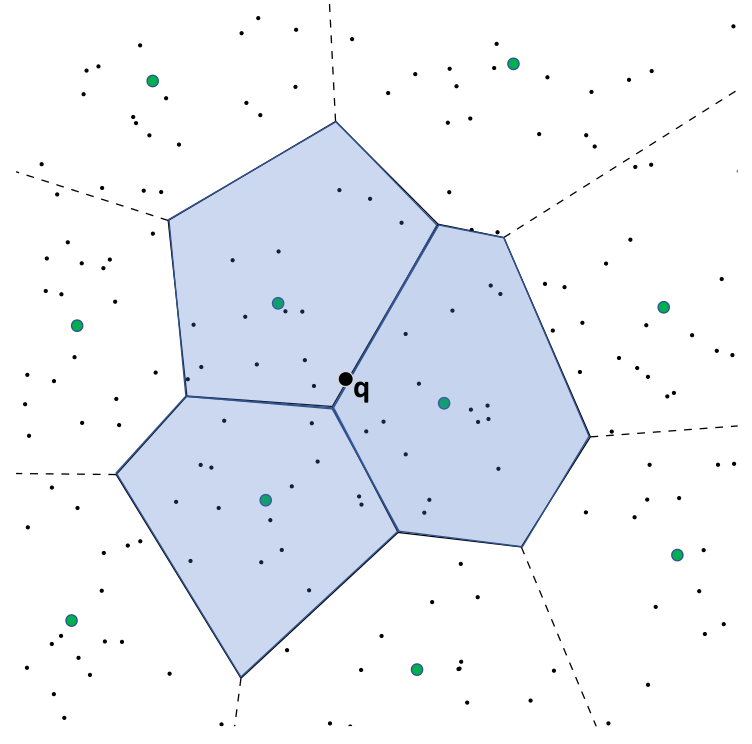
\includegraphics[width=1\linewidth]{Images/Index.png}
\caption{Индексная структура. Зеленым цветом обозначены центроиды ячеек. Черная точка $q$ — запрос поиска. Синим цветом выделены ближайшие ячейки, вектора которых попадают в список кандидатов.}
\label{ris:index}
\end{minipage}
\hfill
\begin{minipage}[h]{0.48\linewidth}
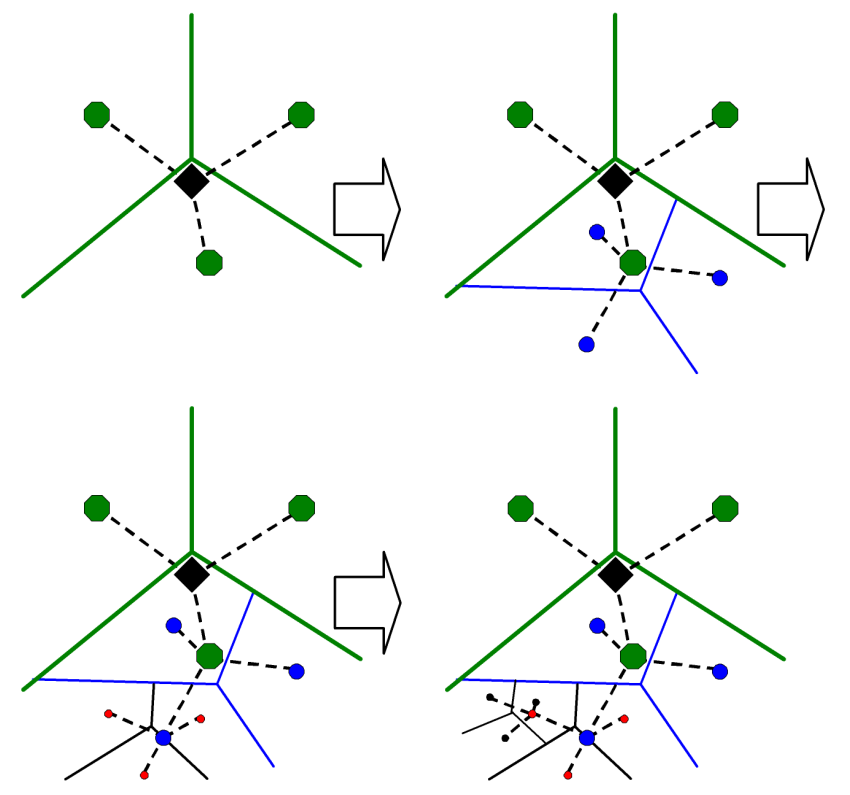
\includegraphics[width=1\linewidth]{Images/HierarchicalIndex.png}
\caption{Иерархический индекс. Процесс построения иерархического инвертированного индекса с разбиением на $K$ ячеек ($K$ = 3). На рисунке представлено четырехуровневое разбиение.}
\label{ris:hierachicalindex}
\end{minipage}
\end{figure}

В связи с этим более подробно обсудим алгоритмы индексирования, основанные на квантовании. Так как полное сравнение вектора запроса со всеми векторами коллекции невозможно, список кандидатов нужно сокращать. Поэтому была придумана инвертированная индексная структура для быстрого доступа к наиболее значимым векторам. Общая идея в том, что инвертированый индекс содержит связные списки векторов, где каждый список является отображением некоторого вектора-центроида. На первом этапе запроса определяется центроид, затем по определенному этим вектором списку выполняется исчерпывающий поиск (Рис.~\ref{ris:index}).

Простейший инвертированный индекс основан на векторном квантовании (VQ)~\cite{1,2,7}. Цель VQ -- уменьшить количество элементов представления пространства поиска. Формально VQ -- это функция $q$, отображающая $D$-мерный вектор $x\in R^D$ на вектор $q(x)\in C = \{c_i~|~i\in I\}$, где $I$ -- конечное индексное множество: $I = 0 , ... , k-1$. Вектора $c_i$ называются центроидами. Множество $V_i$ векторов, отображаемых в данный кластер с номером $i$, называется ячейкой Вороного и определяется так:
$$V_i = \{x\in R^D~|~q(x)=c_i\}.$$
Ячейки VQ образуют разбиение пространства поиска. Все векторы, лежащие в одной и той же ячейке $V_i$, представляются одним и тем же центроидом $c_i$. Качество VQ обычно измеряется по среднеквадратичной ошибке между вектором запроса $x$ и его значением $q(x)$:
$$MSE(q) = \mathbb{E}~d(q(x), x)^2,$$
где $d(x, y) = \| x - y \|$ -- евклидово расстояние между $x$ и $y$.
Стандартным методом обучения центроидов VQ является алгоритм кластеризации $K$-средних, который находит оптимальное разбиение путем итеративного сопоставления векторов центроидам и перестройки этих центроидов по сопоставленным векторам.

Поиск по данной структуре производится в два этапа:
\begin{enumerate}
\item Поиск ближайшего к запросу центроида по короткому списку центроидов;
\item Поиск по списку кандидатов, соответствующих этому центроиду.
\end{enumerate}

\begin{figure}[h]
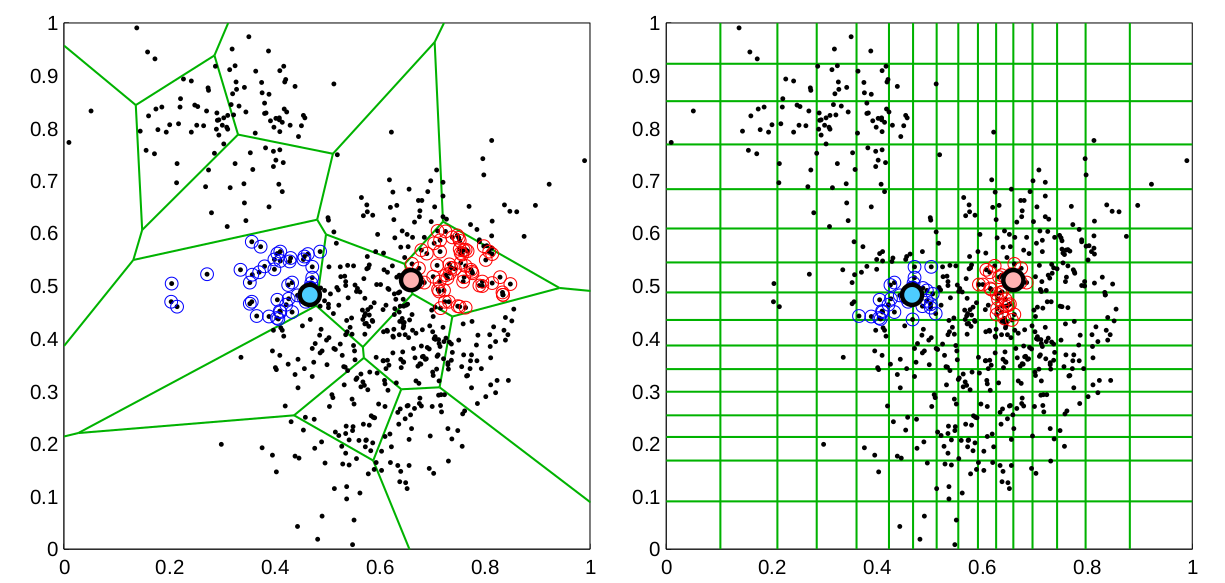
\includegraphics[width=1\linewidth]{Images/MultiIndex.png}
\caption{Левый -- инвертированный индекс. Правый -- инвертированный мульти-индекс. На рисунках представлена разница в разбиении одного и того же набора данных из 600 векторов для разных структур. Для наглядности размерности векторов равны двум. Обе структуры разбивались на 16 ячеек (для каждой размерности). Для примера обозначим два запроса к базе данных, которые отмечены синим и красным цветом. На левом рисунке списки кандидатов содержат 45 и 62 вектора соответственно. Обратим внимание, когда запрос лежит вблизи границы, список кандидатов получается «перекошенным». Для тех же запросов к мульти-индексной структуре списки получаются короче -- 31 и 32 вектора соответственно. Это связанно с тем, что каждая ячейка содержит меньшее количество векторов. Выбирая несколько близких ячеек, можно добиться более точного списка кандидатов.}
\label{ris:multiindex}
\end{figure}

Чтобы обеспечить высокую скорость поиска с использованием инвертированного индекса, количество ячеек должно быть достаточно велико, что сильно снижает скорость обучения алгоритма на больших объемах данных.

Повысить эффективность этапа обучения можно с помощью инвертированного иерархического индекса (HKM)~\cite{11}, который помимо первичного разбиения на ячейки Вороного разбивает пространство каждой ячейки повторно (Рис.~\ref{ris:hierachicalindex}). В огромных датасетах уровень вложенности разбиения выбирается достаточно большим, что гарантирует небольшой список кандидатов. Помимо скорости обучения, при правильном подборе параметров можно добиться ускорения поиска~\cite{11}.

Еще одна идея использования индексов для быстрого поиска предлагает разбивать пространство векторов на несколько подпространств меньшей размерности и обучать каждое подпространство малой размерности отдельно. Это позволяет разбивать датасет на огромное количество ячеек и с помощью декартова произведения центроидов быстро получать доступ к ним (Рис.~\ref{ris:multiindex}). Данная структура называется инвертированным мульти-индексом (IMI)~\cite{3}.

Более формально IMI основан на квантовании произведения (PQ)~\cite{2}, которое представляет из себя схему сжатия с потерями. PQ кодирует каждый вектор $x\in R^D$ как объединение $M$ $\frac{D}{M}$-мерных центроидов из списков $C_1,..., C_M$, каждый из которых содержит $K$ кодовых слов. Другими словами, PQ разбивает вектор на $M$ отдельных подвекторов и применяет векторное квантование (VQ) к каждому подвектору, используя при этом отдельный список центроидов. Следовательно процесс обучения IMI схож с процессом обучения обычного инвертированного индекса, за тем лишь исключением, что обучать приходится несколько списков центроидов. В результате каждый вектор $x$ кодируется набором индексов $[i_1,..., i_M]$ и аппроксимируется как $x \approx [C_1 (i_1),...,C_M (i_M)]$. Быстрое вычисление евклидова расстояния становится возможным благодаря эффективному асиметричному вычислению расстояния~\cite{2} с использованием обученных центроидов:
$$\|x - y\|^2 \approx \|x - [C_1 (i_1),..., C_M(i_M)]\|^2 = \sum_{m=1}^M\|x_m - C_m(i_m)\|^2,$$
где $x_m$ -- составляющая $m$-го подпространства вектора $x$. С точки зрения геометрии PQ эффективно разделяет исходное векторное пространство на $K^M$ ячеек, каждая из которых является декартовым произведением $M$ ячеек меньшей размерности. Однако стоит учитывать, что из-за огромного количества кластеров в IMI некоторые области могут содержать сравнительно малое количество кандидатов или не содержать совсем. Следовательно, IMI в процессе поиска тратит много времени на посещение пустых областей. Причина этого недостатка состоит в том, что IMI при обучении не учитывает зависимость подпространств, которые зачастую зависимы на практике. В частности, существуют значительные корреляции между различными подпространствами дескрипторов, построенных с помощью сверточных нейронных сетей, которые наиболее актуальны в наши дни. Для решения проблемы адаптации алгоритмов к коррелированным данным можно предварительно производить ортогональные преобразования над данными~\cite{4,6} или локальные оптимизации PQ~\cite{5}.